%%%%%%%%%%%%%%%%%%%%%%%%%%%%%%%%%%%%%%%%%%%%%%%%%%%%%%%%%%%%%%%%%%
%%%%%%%% ICML 2014 EXAMPLE LATEX SUBMISSION FILE %%%%%%%%%%%%%%%%%
%%%%%%%%%%%%%%%%%%%%%%%%%%%%%%%%%%%%%%%%%%%%%%%%%%%%%%%%%%%%%%%%%%

% Use the following line _only_ if you're still using LaTeX 2.09.
%\documentstyle[icml2014,epsf,natbib]{article}
% If you rely on Latex2e packages, like most moden people use this:
\documentclass{article}

% use Times
\usepackage{times}
% For figures
\usepackage{graphicx} % more modern
%\usepackage{epsfig} % less modern
%\usepackage{subfigure}

% For citations
\usepackage{natbib}

% For algorithms
\usepackage{algorithm}
\usepackage{algorithmic}

% As of 2011, we use the hyperref package to produce hyperlinks in the
% resulting PDF.  If this breaks your system, please commend out the
% following usepackage line and replace \usepackage{icml2014} with
% \usepackage[nohyperref]{icml2014} above.
\usepackage{hyperref}

% Packages hyperref and algorithmic misbehave sometimes.  We can fix
% this with the following command.
\newcommand{\theHalgorithm}{\arabic{algorithm}}

% Employ the following version of the ``usepackage'' statement for
% submitting the draft version of the paper for review.  This will set
% the note in the first column to ``Under review.  Do not distribute.''
\usepackage{icml2014} 


% The \icmltitle you define below is probably too long as a header.
% Therefore, a short form for the running title is supplied here:
\icmltitlerunning{Objected Recognition based on learning}

\begin{document} 

\twocolumn[
\icmltitle{Objects Recognization Based on On-line Machine Learning\\Project Status Report for CIS 519}

% It is OKAY to include author information, even for blind
% submissions: the style file will automatically remove it for you
% unless you've provided the [accepted] option to the icml2014
% package.
\icmlauthor{Shangyi Cheng}{shangyi@seas.upenn.edu}
\icmlauthor{Yao Chu}{chuyao@seas.upenn.edu}
\icmlauthor{Chenyang Zhao}{chzhao@seas.upenn.edu}

% You may provide any keywords that you 
% find helpful for describing your paper; these are used to populate 
% the "keywords" metadata in the PDF but will not be shown in the document
\icmlkeywords{machine learning, circle detection, feature extraction, objects recognization, neural network}

\vskip 0.3in
]

\begin{abstract} 
So far, we attempted to use following method described in this report to recognize objects (various kinds of balls in our project) in the given images. The first step is using Circular Hough Tansform (CHT) to detect the most possible region that contains the ball which is datasets preprocessing step. The second step contains techniques to extract feature from the selected region. In the third step, neural network is applied on the extracted features to classify the given instances. Several training/testing experiments have be carried out to show the performance of this method.
\end{abstract}


\section{Introduction}

This report presents an attempt of objects recognition. We decided to use images of four kinds of balls from Caltech 256(Griffin, G. Holub, AD. Perona, P.) as our dataset, which contains 98 images of golf in the folder ``088.golf-ball'', 174 in ``193.soccer-ball'', 104 in ``017.bowling-ball'' and 98 in ``216.tennis-ball''.\\
Primary tasks for this project:
\begin{enumerate}
\item Preprocess the datasets and extract the picture patches with different labels. So far, CHT was applied to test the geometric feature of the balls.
\item Based on machine learning method (e.g. Neural Network) to train the datasets.
\item In the test part, input a test image, the algorithm should detect balls in the image and label the detected ball based on the trained model. 
\end{enumerate}

\section{Model Details} 


\subsection{Overview of the Method}
The method for ball recognization is shown in Figure \ref{fig:overview}. Ball recognization can be considered as the problem of detecting the interested region (ball region) in the image, then fetch features inside the interested region as input features for next step. Then label the interested region based on the machine learning classifier (e.g. Neural Network).
\begin{figure}[htp]
\centering
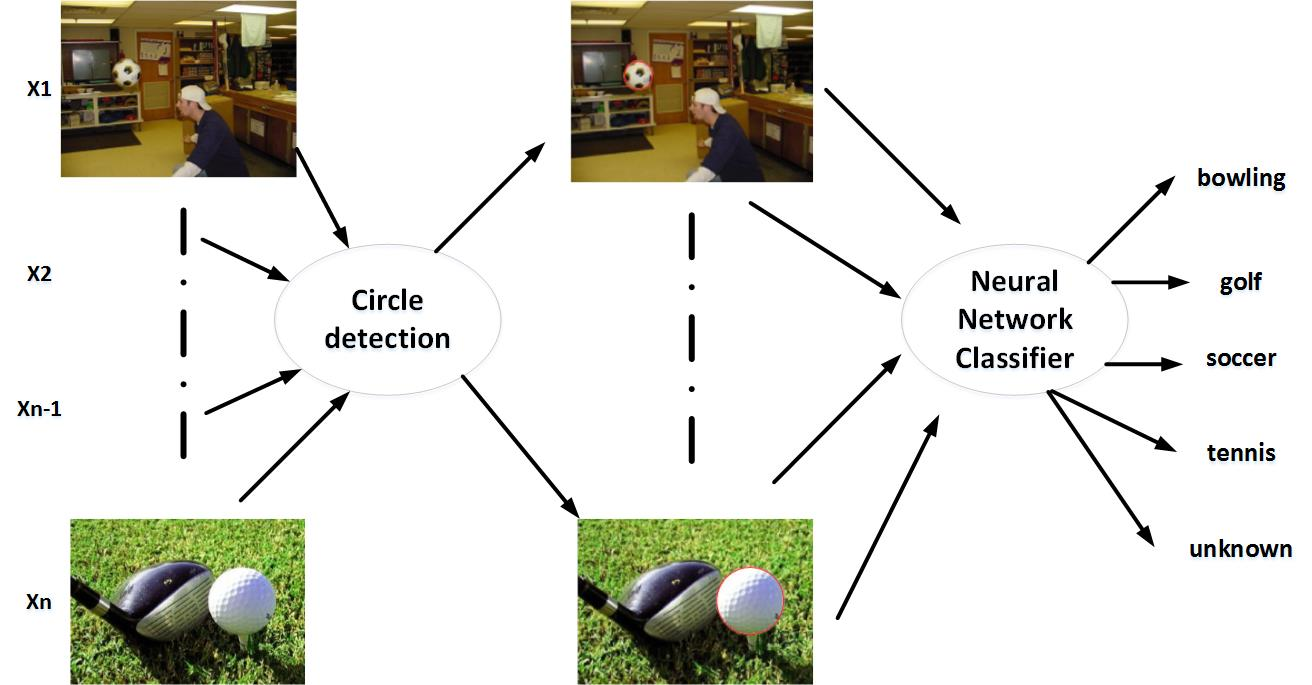
\includegraphics[width=0.4\textwidth]{overview.jpg}
\caption{Methodology Overview}
\label{fig:overview}
\end{figure}

\subsection{Circle Detection}
At the beginning, we considered using corner detection directly on the original image to extract features. However, extracting the corner feature based on the Harris Corner Detection and Adaptive Non-maximal Suppression method\cite{brown2005multi} is not so helpful for following reasons: Firstly, different pattern could be find in a single kind of balls so that geometric corner feature couldn't provide enough information for clssifying; Secondly, the complicated background could generate large amount of features which are irrelevant to the ball. 


During building the training set, the area can be located by either circle detection algorithm or manually selection. However, when classifying a ball in a new image, the circle area has to be detected automatically. Several methods for circle detection are studied in the last few years,\cite{cirDetect1},\cite{cirDetect2},\cite{cirDetect3}. One of the robustest approach is Circle Hough Transform(CHT), which takes the image $M$ and desired radius range $[r_{min},r_{max}]$ as inputs and return the positions of circle centers. The algorithm could be presented in Algorithm \ref{alg:CHT}. In our case, we use the log phase for the accumulator which is
\begin{equation}
\phi_{m,n}^{logr} = 2\pi\Big(\frac{\log{[\sqrt{(m-i)^2+(n-j)^2)}]}-\log{r_{min}}}{\log{r_{max}}-\log{r_{min}}}\Big)
\end{equation}
\begin{algorithm}[tb]
   \caption{Circle Hough Transform}
   \label{alg:CHT}
\begin{algorithmic}
   \STATE {\bfseries Input:} image $I$, radius range $[r_{min},r_{max}]$
   \STATE Initialize accumulator matrix $M = 0$.
   \FOR{each edge point$(i,j)$ in image $I$}
   \FOR{each point $(m,n)$ in image $I$}
   \IF{$r_{min}^2<(m-i)^2+(n-j)^2<r_{max}^2$}
   \STATE {$M(m,n) = M(m,n)+\phi_{m,n}$}
   \ENDIF
   \ENDFOR
   \ENDFOR
   \STATE {\bfseries Return:} positions of local maximum points in accumulator matrix $M$
\end{algorithmic}
\end{algorithm}\\
While applying CHT method, the sensitivity factor is often introduced, which is a scaler in $[0,1]$. A higher sensitivity factor helps in detecting weaker and partially obscured circles, however, increases the risk of false detection. In our case, we increased the sensitivity gradually until the first circle is detected to decrease the risk of false detection and miss detection.

\subsection{Results}
Figure \ref{fig:crd} are some results of our implementation of corner detection, red dots are the detected corners.\\
\begin{figure}[htp]
\centering
	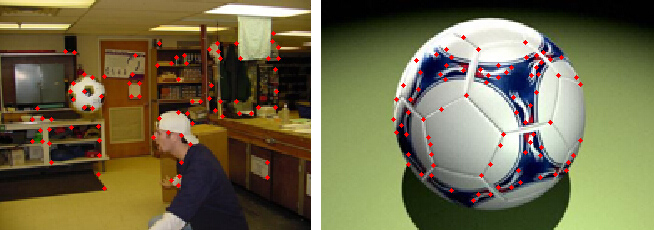
\includegraphics[width=0.4\textwidth]{CornerDetection.jpg}
\caption{Corner Detection Results}
\label{fig:crd}
\end{figure}
Several results of applying our circle detection algorithm on Caltech256 dataset are shown in Figure \ref{fig:cird}.
\begin{figure}[htp]
\centering
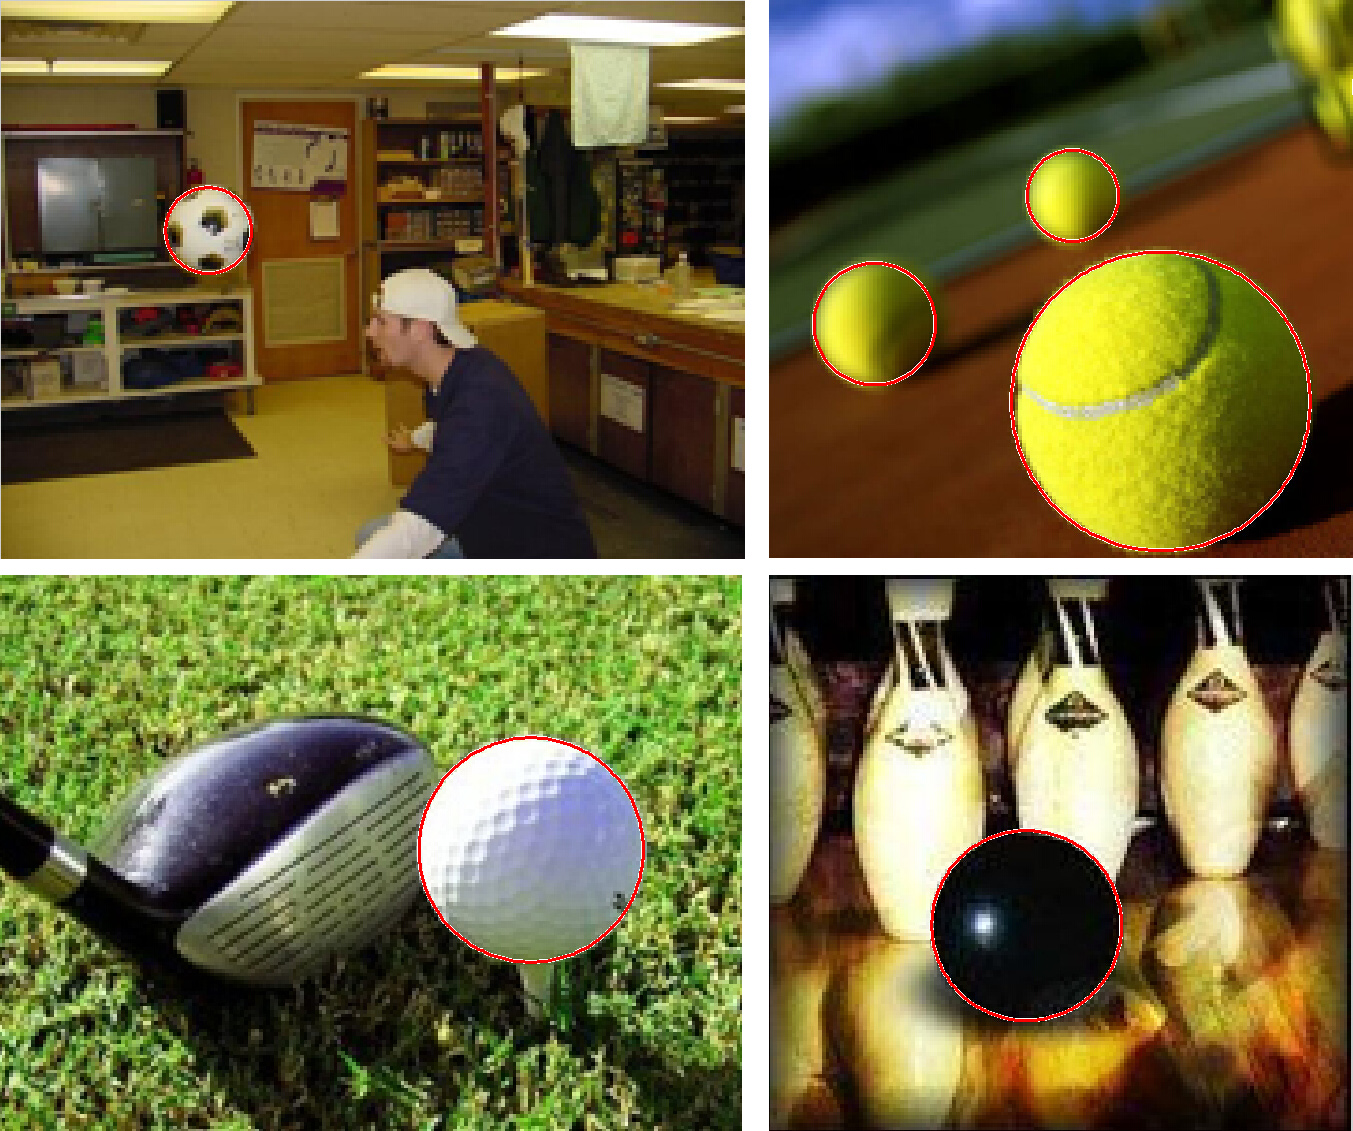
\includegraphics[width=0.4\textwidth]{circleDetection.jpg}
\caption{CHT Detection Result}
\label{fig:cird}
\end{figure}
\section{Work for Next Stage} 

\subsection{Reconstruct the dataset}
In order to introduce neural network into this problem, the training date set need to be normalized to a $n-d$ matrix, where $n$ is the number of training instance and $d$ is the number of pixels. The idea is to resize the intersted area into a particular size, convert the resized image into grey scale and reshape the pixel information into a vector for each circle we found in the circle detection step. Then construct a binary label vector manually according to which kind of ball each instance belongs to.

\subsection{Neural Network learning and Deep learning}
Given all the dataset and the labels, train the classification model by Neural Network learning and Deep learning with cross validation and try to figure out which method is better for ball classification problem. To evaluate the performance of each learning methods, we plans to compute the overall accuracy and precision, recall for each class and plot the ROC curve.

\subsection{HOG and SVM}
So far, CHT has been used to detect the circle, however the result is unreliable in some cases. Inspired by paper presented\cite{dalal2005histograms} by Navneet Dalal and Bill Triggs, we may try the method described in the paper. The interested region will be labeled manually for the training data. HOG features can be extracted from the interested region. Then SVM or other classifier will be applied to train the learning model. 

\section*{Acknowledgments} 
This project is supported by Upenn CIS 519. Thanks Eric Eaton and Xiaoxiang Hu for their instruction. Thanks MATLAB for providing some many useful toolbox.

\bibliography{status-ChengChuZhao}
\bibliographystyle{icml2014}

\end{document} 


